\documentclass[11pt,fleqn]{article}
\usepackage{uebungen}
\renewcommand{\logo}{
\includegraphics[height=10ex]{kit_logo_de_1c_schwarz}}

\usepackage{amsfonts}
\usepackage[dvipsnames]{xcolor}
\usepackage[hidelinks,colorlinks=true,linktocpage=true,linkcolor=NavyBlue,urlcolor=NavyBlue,citecolor=NavyBlue]{hyperref}
%\usepackage[hang]{subfigure}
\usepackage{lmodern}
%\usepackage[scaled=.85]{beramono}
\usepackage{listings}

\usepackage{cleveref}

%\usepackage{caption}
\usepackage{subcaption}
\usepackage{graphicx}

\usepackage{amsmath}
\usepackage{amsthm}
\newtheorem{definition}{Definition}
\newtheorem{lemma}{Lemma}

\usepackage{todonotes}

\definecolor{shellBack}{rgb}{0.95,0.95,0.9}
\lstset{basicstyle=\ttfamily, backgroundcolor=\color{shellBack}}

\def\published{true}

\begin{document}

\kopfBlatt{Neural Network Verification (Exercises 1)}

\section*{DNNV}

For verifying neural networks we will be using the tool \href{https://github.com/dlshriver/dnnv}{\texttt{DNNV}} which provides an accessible platform to execute numerous neural network verification tools and a straightforward specification language.

A comprehensive documentation of \texttt{DNNV} can be found \href{https://docs.dnnv.org/en/stable/}{online}, but for a reference we go through a simple example as part of the exercise.
This simple example should provide you with all the knowledge you need to master the exercises of this class.

\subsection*{Installation}
None.\\
Instead of installing \texttt{DNNV} and its dependencies on your machine, you can use the tool directly within \href{https://hub.bwjupyter.de}{\textbf{bwJupyter}}.
To this end, first login to bwjupyter. Subsequently, click on the following link:

\begin{center}
\href{https://hub.bwjupyter.de/services/profilemanagement/add?profile=1dc4ab7f-99d3-44d6-9f64-eb7eee1f4ee5}{https://hub.bwjupyter.de/services/profilemanagement/\\add?profile=1dc4ab7f-99d3-44d6-9f64-eb7eee1f4ee5}\\
\end{center}

This should add a profile called \textbf{``Formale Systeme II: Anwendung (SoSe 2025) - NN Verifikation''} to the set of available Jupyter Lab environments.
Subsequently head to the \href{https://hub.bwjupyter.de/hub/home}{``Home''} page, click ``Start My Server'' and choose this profile clicking ``Start'' (if you clicked on the link above first, you should see this profile under ``Shared Profiles'').
After a short while a Juypter Lab environment should pop up in your browser window.

\subsection*{A ``Hello World'' example.}
To get started, we have generated a very small neural network in \texttt{\_\_shared/nets/at\_least.onnx}.
To check whether your setup is working, open a terminal inside your jupyter lab and enter the following command:
\begin{center}
\texttt{dnnv --mipverify --mipverify.optimizer=GLPK -N N \_\_shared/nets/at\_least.onnx \_\_shared/props/at\_least.py}
\end{center}
This command does a few things:
\begin{itemize}
    \item \texttt{-mipverify} configures \texttt{DNNV} to use the NN verifier \href{https://github.com/vtjeng/MIPVerify.jl}{\texttt{MIPVerify}} which encodes the NN as a MILP problem (simiar to what we saw in the lecture)
    \item \texttt{--mipverify.optimizer=GLPK} configures \texttt{MIPVerify} to use the MILP solver GLPK
    \item \texttt{-N N \_\_shared/nets/at\_least.onnx} tells \texttt{DNNV} that the neural network \texttt{N} (which we will be referencing in our specification) can be found in the ONNX file \texttt{\_\_shared/nets/at\_least.onnx}
    \item \texttt{\_\_shared/props/at\_least.py} provides \texttt{DNNV} with the specification to verify.
\end{itemize}
\texttt{DNNV} should run for approximately 30 seconds before returning with the result \textit{unsat}.

\subsection*{Understanding what just happened}
Before we try to specify and verify a few neural networks of our own, let's first understand what just happened:
%https://raw.githubusercontent.com/samysweb/nn-verification-101/refs/heads/main/provided/nets/at_least.onnx
\begin{enumerate}
    \item You can inspect the neural network using the online tool \texttt{Netron} \href{https://netron.app/?url=https://raw.githubusercontent.com/samysweb/nn-verification-101/refs/heads/main/provided/nets/at_least.onnx}{under this link}:
    You see a combined matrix multiplication and bias addition (\textbf{Ge}neralized\textbf{M}atrix\textbf{M}ultiplication), an application of a ReLU function, and another GeMM operation.
    Clicking on on one of the parameters of the operations (e.g. \textbf{B} of the first GeMM) opens a sidebar with further information on the parameters.
    Click on the white area next to ``value'' to see the NN's concrete parameters.\\
    Inspect the parameters: Do you have a hypothesis what behaviour this NN is exhibiting?
    \item Inspect the specification in \texttt{\_\_shared/props/at\_least.py}:
    \begin{itemize}
        \item Did you expect this property to be satisfies based on your manual inspection of the weights?
        \item Note the file specifices a property that is universally quantified.\\
        In today's lecture you heard about two different, dual, formulations for NN verification.\\
        Recall what you learned about encoding NN verification problems as MILP problems today:
        How do you think does \texttt{DNNV} reformulate the property before sending it to the low-level solver?
    \end{itemize}
    \item Run \texttt{DNNV} with the additional argument \texttt{-v} after ``\texttt{CONJUNCTION:}'' this prints the concrete queries that are being sent to the low-level verification tool.\\
    Check if \texttt{DNNV} modified the query in the way that you had expected.
\end{enumerate}

\section*{Guaranteeing Functional Correctness}
In the section below ("Airborne Collision Avoidance Properties") we have provided you with some properties.
Under \texttt{\_\_shared/nets/} you find some NNs for an Airborne Collision Avoidance System.
Use these NNs to verify some of the properties formulated below.

\section*{Robutness to image perturbations}

% dnnv -v --eran --eran.domain deepzono -N N __shared/nets/mnist_convnn_aug.onnx __shared/solutions/mnist-0.py
% UNSAT


\clearpage
\section*{Airborne Collision Avoidance Properties}

In this exercise you are supposed to encode properties that are desirable for an
Airborne Collision Avoidance System.
This system provides guidance to a pilot in situations where two planes are approaching each other and there is a risk for a \emph{Near Mid Air Collision} (closer than 100ft vertically and 500ft horizontally).
This exercise concerns itself with \emph{horizontal} collision avoidance, i.e. we assume the planes 
are inevitably approaching a point where they are no longer vertically separated.
The plane of the pilot that our system is providing advice to is called the \emph{ownship} while the other plane is called \emph{intruder}.


\begin{figure}
    \centering
    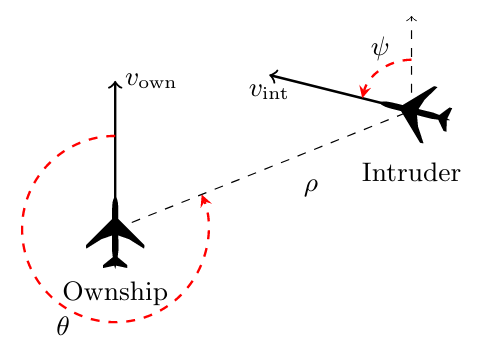
\includegraphics[width=0.35\textwidth]{figures/acas.png}
    \caption{Geometry for Horizontal Airborne Collision Avoidance (taken from Katz et al. 2017)}
    \label{fig:acas}
\end{figure}

\paragraph*{Inputs}
The inputs of the Airborne Collision Avoidance System are as follows (see also \Cref{fig:acas})
\begin{enumerate}
    \item $\rho \in \left[0,60\,000\right]$: Distance to Intruder in m
    \item $\theta \in \left[-\pi,\pi\right]$: Angle to intruder rel. to ownship (in radians)
    \item $\psi \in \left[-\pi,\pi\right]$: Heading angle of intruder rel. to ownship (in radians)
    \item $v_{\text{own}} \in \left[100,1200\right]$: Speed of ownship in m/s
    \item $v_{\text{int}} \in \left[0,1200\right]$: Speed of intruder in m/s
    \item $\alpha_{\text{prev}}\in\left\{\text{Clear-of-Conflict}, \text{weak left}, \text{weak right}, \text{strong left}, \text{strong right}\right\}$\\
    The advisory given by the NN in the previous time step.
    \item $\tau \in \left\{0, 1, 5, 10, 20, 40, 60, 80, 100\right\}$: Time until loss of vertical separation
\end{enumerate}
The first 5 inputs are given to the NN.
For every possible instantiation of the last two inputs (e.g. for $\alpha_{\text{prev}}=\text{Clear-of-Conflict}$ $\tau=100$) there exists a specific neural network.


\paragraph*{Output.}
For each of the possible five actions (in order: Clear of Conflict, Weak Left, Weak Right, Strong Left, Strong Right),
the NN outputs a score.
The minimal score then determines the next advisory.

\paragraph*{Input Normalization.}
The inputs of the neural network need to be normalized using the following formula w.r.t. a given mean $M$ and given range $R$:
\[
\hat{x} = \frac{x - M}{R}
\]
The values for $R$ and $M$ are in \Cref{tab:acas_normalization}.
%1.9791091e+04,0.0,0.0,650.0,600.0,7.5188840201005975,
%60261.0,6.28318530718,6.28318530718,1100.0,1200.0,373.94992,
\begin{table}[h]
\caption{Input normalization for ACAS NNs}
\centering
\begin{tabular}{l|l|l}
    \textbf{Input} & $\mathbf{M}$ & $\mathbf{R}$\\\hline
    $\rho$ & 1979 & 60261\\
    $\theta$ & 0.0 & $2\pi$\\
    $\psi$ & 0.0 & $2\pi$\\
    $v_{\text{own}}$ &  650 & 1100\\
    $v_{\text{int}}$ &  600 & 1200\\
\end{tabular}
\label{tab:acas_normalization}
\end{table}


The output scores must uniformly be \emph{denormalized} as follows:
\[
y = 373.94992*\hat{y}+7.5188840201005975
\]

\subsection*{Properties}
Here we describe properties of interest for the ACAS System.
Choose some of these properties and verify them on suggested NNs:

% \paragraph*{Property 1}
% If the intruder is more than 55947m away and the ownship is at least 1085 m/s \emph{faster},
% then the score for Clear of Conflict is at most 1500.

% \textit{Hint 1:}: DNNV does not directly support linear constraints over multiple input variables.\\
% If you cannot encode the property directly, try to encode a requirement using the
% variable's known bounds that is necessary or sufficient.

% """
% Property $\phi_1$.
%   - Description: If the intruder is distant and is significantly slower than the ownship, the score of a COC advisory will always be below a certain fixed threshold.
%   - Tested on: all 45 networks.
%   - Input constraints: $\rho \ge 55947.691$, $v_{own} \ge 1145$, $v_{int} \le 60$.
%   - Desired output property: the score for COC is at most 1500.
% """

\paragraph*{Property 2}
Assume the intruder is 1500-1800 meters away and directly ahead ($\pm 3$ degrees).
If the intruder is flying directly towards the ownship ($\pm 3$ degrees),
the score for Clear of Conflict will not be minimal.

\textit{Hint 1:} Assume the ownship is flying with at least 980 m/s and the intruder with at least 960 m/s.

\textit{Hint 2:} You may use \texttt{np.argmin}

\textit{Hint 3:} At 180 degrees there is an ``overflow'' in radians from positive to negative values.
You may split up your query into multiple queries and/or only focus on the positive case for starters.

\textit{Suggested NN:} ACAS\_2\_1.onnx ($\alpha_{\text{prev}}=\text{weak left}$, $\tau=0s$)

% """
% Property $\phi_3$.
%   - Description: If the intruder is directly ahead and is moving towards the ownship, the score for COC will not be minimal.
%   - Tested on: all networks except $N_{1,7}$, $N_{1,8}$, and $N_{1,9}$.
%   - Input constraints: $1500 \le \rho \le 1800$, $-0.06 \le \theta \le 0.06$, $\psi \ge 3.10$, $v_{own} \ge 980$, $v_{int} \ge 960$.
%   - Desired output property: the score for COC is not the minimal score.
% """

\paragraph*{Property 4}
If the intruder is directly ahead (1500-1800 m away; $\left|\theta\right|$ negligible) and is moving away from the ownship in a straight line, but at a significantly lower speed than the ownship (at least 200 m/s less), then the network will not suggest Clear of Conflict.

\textit{Hint 1:} You may use \texttt{np.argmin}

\textit{Hint 2:} Assume that $v_{\text{own}} \geq 1000$ and $v_{\text{int}} \geq 700$

\textit{Suggested NN:} ACAS\_2\_9.onnx ($\alpha_{\text{prev}}=\text{weak left}$, $\tau=100s$)

%   - Description: If the intruder is directly ahead and is moving away from the ownship but at a lower speed than that of the ownship, the score for COC will not be minimal.
%   - Tested on: all networks except $N_{1,7}, $N_{1,8}$, and $N_{1,9}$.
%   - Input constraints: $1500 \le \rho \le 1800$, $-0.06 \le θ \le 0.06$, $\psi = 0$, $v_{own} \ge 1000$, $700 \le v_{int} \le 800$.
%   - Desired output property: the score for COC is not the minimal score.



\paragraph*{Property 2}
If the intruder is further than 55947 m away and the ownship is at least 1085 m/s \emph{faster}
than the intruder, the Clear of Conflict score is not the maximal one.

\textit{Hint 1:}
\texttt{DNNV} does not easily support to directly encode linear constraints over input variables.
Instead, try an interval-based formulation that could help you find counterexamples.

\textit{Hint 2:}
In case \texttt{DNNV} returns SAT you can save the counterexample as a numpy array using \texttt{--save-violation YOUR\_PATH}.
You can inspect the counterexample via:\\
\texttt{
import numpy as np
print(np.load(YOUR\_PATH))
}

\textit{Suggested NN:} ACAS\_2\_1.onnx ($\alpha_{\text{prev}}=\text{weak left}$, $\tau=0s$)

% """
% Property $\phi_2$.
%   - Description: If the intruder is distant and is significantly slower than the ownship, the score of a COC advisory will never be maximal.
%   - Tested on: $N_{x,y}$ for all $x \ge 2$ and for all $y$.
%   - Input constraints: $\rho \ge 55947.691$, $v_{own} \ge 1145$, $v_{int} \le 60$.
%   - Desired output property: the score for COC is not the maximal score.
% """

% \paragraph{Property 9}
% Even if the previous advisory was ``weak right'', the presence of a \emph{nearby intruder}
% will cause the network to output a ``strong left'' advisory instead.

% To this end, we define the nearby intruder as being 2000-7000 meters away that is 22 to 9 degrees left of the ownship with the intruder flying in inverse direction to the plane.

% \textit{Hint 1:} For starters, consider this property for velocities $\leq 150$ for both parties.

% \textit{Hint 2:} If verification times out, try reducing the range of allowed distance.

% \textit{Suggested NN:} ACAS\_2\_9.onnx ($\alpha_{\text{prev}}=\text{weak left}$, $\tau=100$)

% """
% Property $\phi_9$.
%   - Description: Even if the previous advisory was ``weak right'', the presence of a nearby intruder will cause the network to output a ``strong left'' advisory instead.
%   - Tested on: $N_{3,3}$.
%   - Input constraints: $2000 \le \rho \le 7000$, $-0.4 \le \theta \le -0.14$, $-3.141592 \le \psi \le -3.141592 + 0.01$, $100 \le v_{own} \le 150$, $0 \le v_{int} \le 150$.
%   - Desired output property: the score for ``strong left'' is minimal.
% """

\end{document}

%  LocalWords:  Spielbrett
